% Producción de trigo por departamento, año 2022. Adaptado de MDPyEP (2023),
% Tabla 2 (fuente original: INE con base en OAP--MDRyT). Valores sin modificar.
% NOTA: en la fuente, la suma de los departamentos (310 154 t) no coincide con
% el total publicado (310 730 t), y Potosí figura con 18 655 t y 6,2 %
% (18 655 t equivalen a 6,0 %). Se reproducen los valores tal como constan.
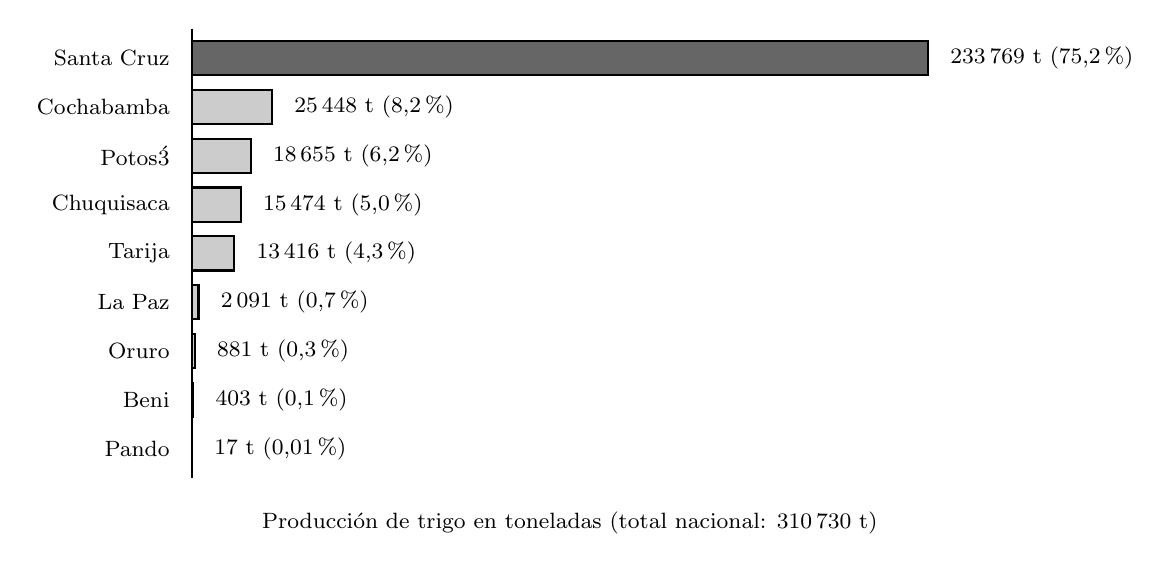
\begin{tikzpicture}[
    x=0.04cm,
    y=-0.62cm,
    barra/.style={draw, fill=black!20, thick},
    destacada/.style={draw, fill=black!60, thick},
    etiqueta/.style={font=\footnotesize, anchor=east},
    valor/.style={font=\footnotesize, anchor=west}
]

% Departamento / producción (miles de t, solo para la longitud de barra) / etiqueta de producción / participación
\foreach \dep/\val/\txt/\por [count=\i] in {
    Santa Cruz/233.769/233\,769/75{,}2,
    Cochabamba/25.448/25\,448/8{,}2,
    Potosí/18.655/18\,655/6{,}2,
    Chuquisaca/15.474/15\,474/5{,}0,
    Tarija/13.416/13\,416/4{,}3,
    La Paz/2.091/2\,091/0{,}7,
    Oruro/0.881/881/0{,}3,
    Beni/0.403/403/0{,}1,
    Pando/0.017/17/0{,}01}
{
    \ifnum\i=1
        \draw[destacada] (0,\i-0.35) rectangle (\val,\i+0.35);
    \else
        \draw[barra] (0,\i-0.35) rectangle (\val,\i+0.35);
    \fi
    \node[etiqueta] at (-4,\i) {\dep};
    \node[valor] at (\val+4,\i) {\txt~t (\por\,\%)};
}

% Eje
\draw[thick] (0,0.4) -- (0,9.6);
\node[font=\footnotesize, anchor=north] at (120,10.1)
    {Producción de trigo en toneladas (total nacional: 310\,730~t)};

\end{tikzpicture}
